% 2-15-rb-tree.tex

%%%%%%%%%%%%%%%%%%%%
\documentclass[a4paper, justified]{tufte-handout}

% hw-preamble.tex

% geometry for A4 paper
% See https://tex.stackexchange.com/a/119912/23098
\geometry{
  left=20.0mm,
  top=20.0mm,
  bottom=20.0mm,
  textwidth=130mm, % main text block
  marginparsep=5.0mm, % gutter between main text block and margin notes
  marginparwidth=50.0mm % width of margin notes
}

% for colors
\usepackage{xcolor} % usage: \color{red}{text}
% predefined colors
\newcommand{\red}[1]{\textcolor{red}{#1}} % usage: \red{text}
\newcommand{\blue}[1]{\textcolor{blue}{#1}}
\newcommand{\teal}[1]{\textcolor{teal}{#1}}

\usepackage{todonotes}

% heading
\usepackage{sectsty}
\setcounter{secnumdepth}{2}
\allsectionsfont{\centering\huge\rmfamily}

% for Chinese
\usepackage{xeCJK}
\usepackage{zhnumber}
\setCJKmainfont[BoldFont=FandolSong-Bold.otf]{FandolSong-Regular.otf}

% for fonts
\usepackage{fontspec}
\newcommand{\song}{\CJKfamily{song}} 
\newcommand{\kai}{\CJKfamily{kai}} 

% To fix the ``MakeTextLowerCase'' bug:
% See https://github.com/Tufte-LaTeX/tufte-latex/issues/64#issuecomment-78572017
% Set up the spacing using fontspec features
\renewcommand\allcapsspacing[1]{{\addfontfeature{LetterSpace=15}#1}}
\renewcommand\smallcapsspacing[1]{{\addfontfeature{LetterSpace=10}#1}}

% for url
\usepackage{hyperref}
\hypersetup{colorlinks = true, 
  linkcolor = teal,
  urlcolor  = teal,
  citecolor = blue,
  anchorcolor = blue}

\newcommand{\me}[4]{
    \author{
      {\bfseries 姓名:}\underline{#1}\hspace{2em}
      {\bfseries 学号:}\underline{#2}\hspace{2em}\\[10pt]
      {\bfseries 评分:}\underline{#3\hspace{3em}}\hspace{2em}
      {\bfseries 评阅:}\underline{#4\hspace{3em}}
  }
}

% Please ALWAYS Keep This.
\newcommand{\noplagiarism}{
  \begin{center}
    \fbox{\begin{tabular}{@{}c@{}}
      请独立完成作业,不得抄袭。\\
      若得到他人帮助, 请致谢。\\
      若参考了其它资料,请给出引用。\\
      鼓励讨论,但需独立书写解题过程。
    \end{tabular}}
  \end{center}
}

\newcommand{\goal}[1]{
  \begin{center}{\fcolorbox{blue}{yellow!60}{\parbox{0.50\textwidth}{\large 
    \begin{itemize}
      \item 体会``思维的乐趣''
      \item 初步了解递归与数学归纳法 
      \item 初步接触算法概念与问题下界概念
    \end{itemize}}}}
  \end{center}
}

% Each hw consists of four parts:
\newcommand{\beginrequired}{\hspace{5em}\section{作业 (必做部分)}}
\newcommand{\beginoptional}{\section{作业 (选做部分)}}
\newcommand{\beginot}{\section{Open Topics}}
\newcommand{\begincorrection}{\section{订正}}
\newcommand{\beginfb}{\section{反馈}}

% for math
\usepackage{amsmath, mathtools, amsfonts, amssymb}
\newcommand{\set}[1]{\{#1\}}

% define theorem-like environments
\usepackage[amsmath, thmmarks]{ntheorem}

\theoremstyle{break}
\theorempreskip{2.0\topsep}
\theorembodyfont{\song}
\theoremseparator{}
\newtheorem{problem}{题目}[subsection]
\renewcommand{\theproblem}{\arabic{problem}}
\newtheorem{ot}{Open Topics}

\theorempreskip{3.0\topsep}
\theoremheaderfont{\kai\bfseries}
\theoremseparator{:}
\theorempostwork{\bigskip\hrule}
\newtheorem*{solution}{解答}
\theorempostwork{\bigskip\hrule}
\newtheorem*{revision}{订正}

\theoremstyle{plain}
\newtheorem*{cause}{错因分析}
\newtheorem*{remark}{注}

\theoremstyle{break}
\theorempostwork{\bigskip\hrule}
\theoremsymbol{\ensuremath{\Box}}
\newtheorem*{proof}{证明}

% \newcommand{\ot}{\blue{\bf [OT]}}

% for figs
\renewcommand\figurename{图}
\renewcommand\tablename{表}

% for fig without caption: #1: width/size; #2: fig file
\newcommand{\fig}[2]{
  \begin{figure}[htbp]
    \centering
    \includegraphics[#1]{#2}
  \end{figure}
}
% for fig with caption: #1: width/size; #2: fig file; #3: caption
\newcommand{\figcap}[3]{
  \begin{figure}[htbp]
    \centering
    \includegraphics[#1]{#2}
    \caption{#3}
  \end{figure}
}
% for fig with both caption and label: #1: width/size; #2: fig file; #3: caption; #4: label
\newcommand{\figcaplbl}[4]{
  \begin{figure}[htbp]
    \centering
    \includegraphics[#1]{#2}
    \caption{#3}
    \label{#4}
  \end{figure}
}
% for margin fig without caption: #1: width/size; #2: fig file
\newcommand{\mfig}[2]{
  \begin{marginfigure}
    \centering
    \includegraphics[#1]{#2}
  \end{marginfigure}
}
% for margin fig with caption: #1: width/size; #2: fig file; #3: caption
\newcommand{\mfigcap}[3]{
  \begin{marginfigure}
    \centering
    \includegraphics[#1]{#2}
    \caption{#3}
  \end{marginfigure}
}

\usepackage{fancyvrb}

% for algorithms
\usepackage[]{algorithm}
\usepackage[]{algpseudocode} % noend
% See [Adjust the indentation whithin the algorithmicx-package when a line is broken](https://tex.stackexchange.com/a/68540/23098)
\newcommand{\algparbox}[1]{\parbox[t]{\dimexpr\linewidth-\algorithmicindent}{#1\strut}}
\newcommand{\hStatex}[0]{\vspace{5pt}}
\makeatletter
\newlength{\trianglerightwidth}
\settowidth{\trianglerightwidth}{$\triangleright$~}
\algnewcommand{\LineComment}[1]{\Statex \hskip\ALG@thistlm \(\triangleright\) #1}
\algnewcommand{\LineCommentCont}[1]{\Statex \hskip\ALG@thistlm%
  \parbox[t]{\dimexpr\linewidth-\ALG@thistlm}{\hangindent=\trianglerightwidth \hangafter=1 \strut$\triangleright$ #1\strut}}
\makeatother

% for footnote/marginnote
% see https://tex.stackexchange.com/a/133265/23098
\usepackage{tikz}
\newcommand{\circled}[1]{%
  \tikz[baseline=(char.base)]
  \node [draw, circle, inner sep = 0.5pt, font = \tiny, minimum size = 8pt] (char) {#1};
}
\renewcommand\thefootnote{\protect\circled{\arabic{footnote}}} % feel free to modify this file
%%%%%%%%%%%%%%%%%%%%
\title{第3-X讲-订正}
\me{林凡琪}{211240042}{}{}
\date{\zhtoday} % or like 2019年9月13日
%%%%%%%%%%%%%%%%%%%%
\begin{document}
\maketitle
%%%%%%%%%%%%%%%%%%%%
\noplagiarism % always keep this line
%%%%%%%%%%%%%%%%%%%%
\begin{abstract}
    % \begin{center}{\fcolorbox{blue}{yellow!60}{\parbox{0.65\textwidth}{\large 
    %   \begin{itemize}
    %     \item 
    %   \end{itemize}}}}
    % \end{center}
\end{abstract}
%%%%%%%%%%%%%%%%%%%%
\beginrequired

%%%%%%%%%%%%%%%




% \vspace{0.50cm}
%%%%%%%%%%%%%%%
% \begin{ot}[]
% 
%   \noindent 参考资料:
%   \begin{itemize}
%     \item 
%   \end{itemize}
% \end{ot}

% \begin{solution}
% \end{solution}
%%%%%%%%%%%%%%%

%%%%%%%%%%%%%%%%%%%%
% 如果没有需要订正的题目,可以把这部分删掉

\begincorrection
%%%%%%%%%%%%%%%%%%%%

\begin{problem}[3-12.3 CZ 8.14]
Prove that a graph G without isolated vertices has a perfect matching if and only if   $\alpha_1(G) = \beta_1(G)$.
\end{problem}

\begin{solution}
    如果$n$阶图$G$有完美匹配,那么最大匹配数=$\beta_1{G}=\frac{n}{2}$.\\
    又因为$\beta_1{G}+\alpha_1{G}=n$,\\
    所以可得 $\alpha_1(G) = \beta_1(G)$.\\
    如果$\alpha_1(G) = \beta_1(G)$,那么$\alpha_1(G) = \beta_1(G)=\frac{n}{2}$\\
    所以图的最大匹配数为$\frac{n}{2}$且完美匹配是存在的.\\
    综上得证.
\end{solution}

%%%%%%%%%%%%%%%

%%%%%%%%%%%%%%%
\begin{problem}[3-12.4 CZ 8.16]
Prove that if G is a graph of order n, maximum degree $\delta$ and having no isolated vertices, then $\beta(G)\geq \frac{n}{\delta + 1}$
\end{problem}

\begin{solution}
    设$G$的最小点覆盖集为:$S$, 同时$T$为$G-S$。\\
    由点覆盖集性质知, $T$包含了$S$在$G$中的全部所连点,所以可知$|T|\leq \delta \times |S|$, 那么$n-\beta(G)\leq \delta \times \beta(G)$\\
    最后可得 $\beta(G)\geq \frac{n}{\delta + 1}$
\end{solution}
%%%%%%%%%%%%%%%

%%%%%%%%%%%%%%%
\begin{problem}[3-12.5 CZ 8.18]
Give an example of a 5-regular graph that contains no 1-factor.
\end{problem}

\begin{solution}
    \newpage
    \begin{figure}[htbp]
        \centering
        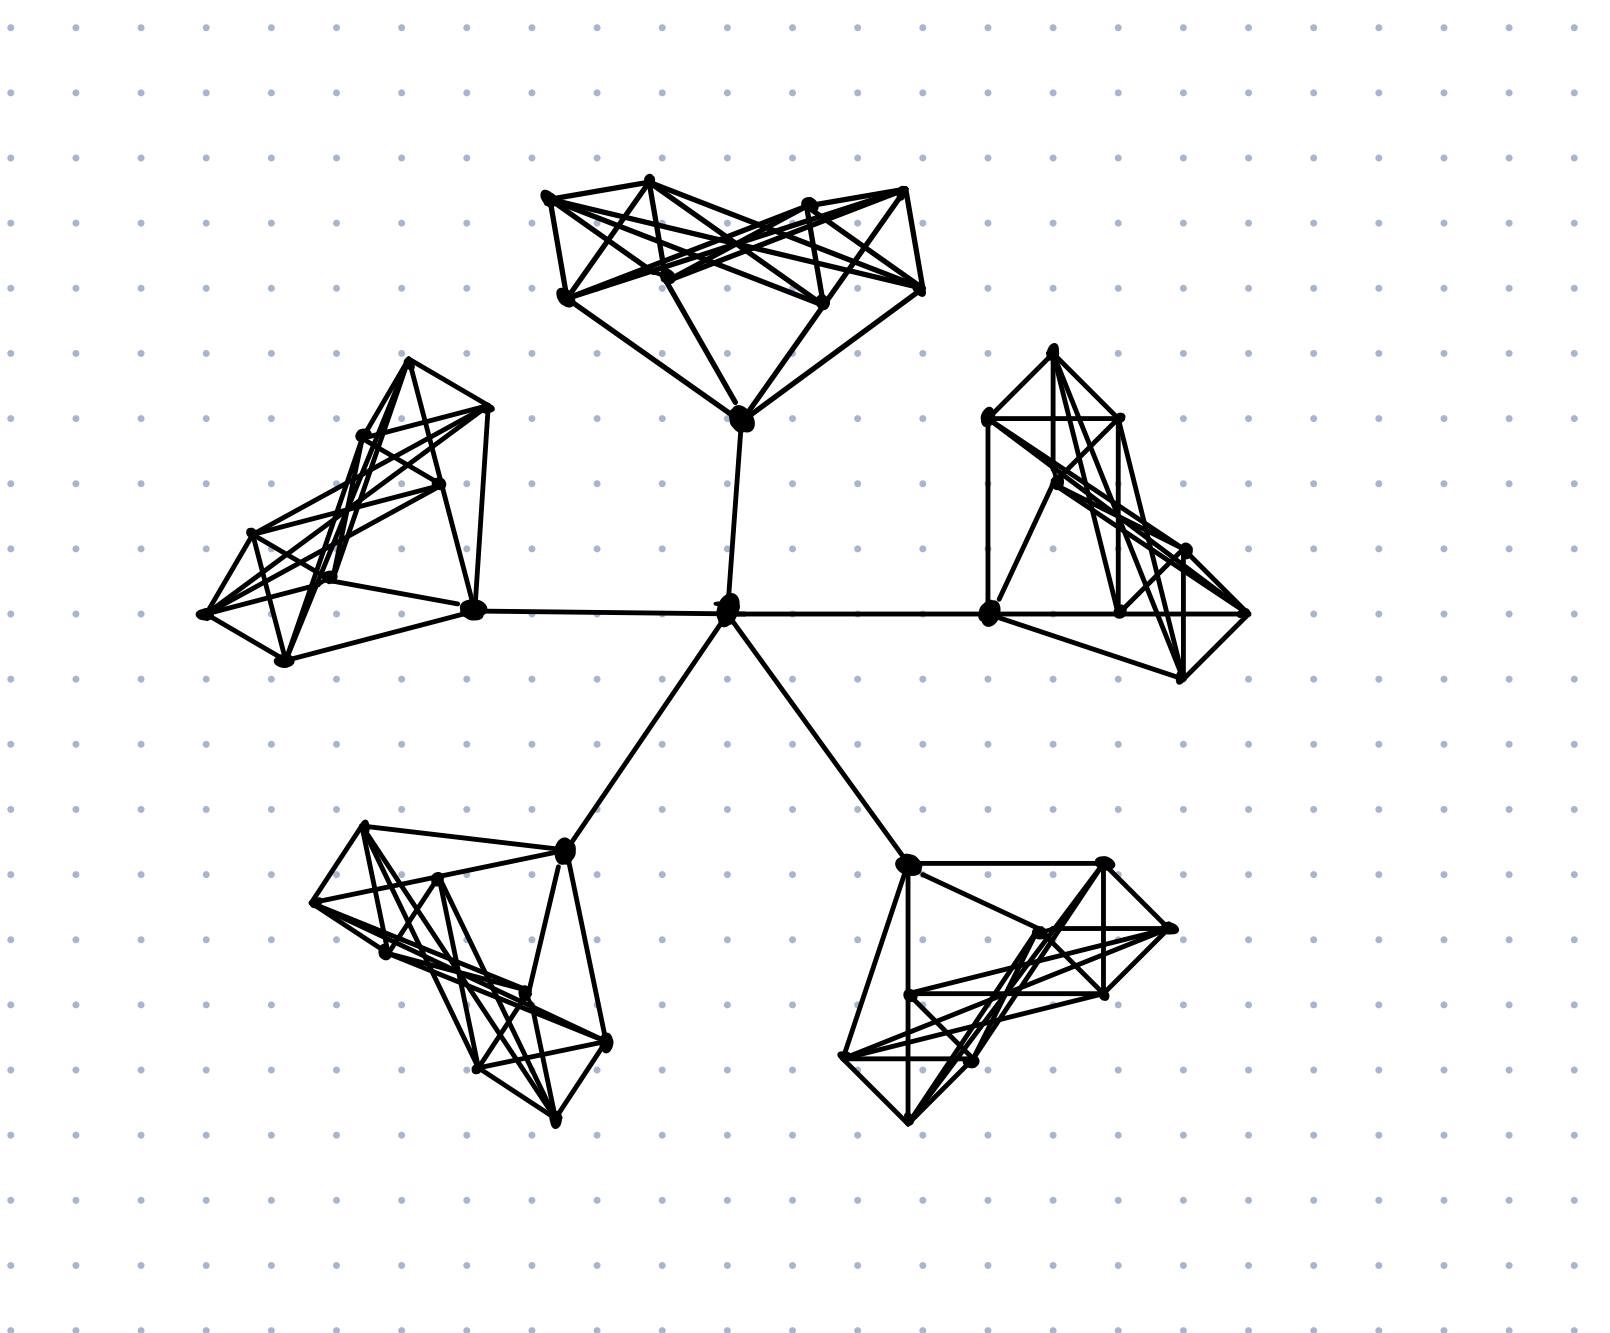
\includegraphics[width = 0.75\linewidth]{5.jpg}
    \end{figure}
\end{solution}

%%%%%%%%%%%%%%%

\begin{problem}[3-7.1 TC 22.1-3]
The \textbf{transpose} of a directed graph $G=(V,E)$ is the graph $G^T=(V,E^T)$, where $E^T=\{(v,u)\in V\times V:(u,v) \in E\}$.Thus,$G^T$ is $G$ with all its edge sreversed. Describe efficient algorithms for computing $G^T$ from $G$, for both the adjacency-list and adjacency-matrix representations of $G$. Analyze the running times of your algorithms.
\end{problem}

\begin{solution}
    \noindent
    \begin{algorithm}
        \caption{adjacency-list}\label{euclid}
        \begin{algorithmic}[1]
            \Procedure{adjacency-list }{V}
            \For {$x \in V$}
            \For{$y \in E(x)$}
            \State add $x$ to $E^{1}(y)$
            \EndFor
            \EndFor
            \EndProcedure
        \end{algorithmic}
    \end{algorithm}
    \noindent
    \noindent
    \begin{algorithm}
        \caption{adjacency-matrix}\label{euclid}
        \begin{algorithmic}[1]
            \Procedure{adjacency-matrix }{V}
            \For {$x \in V$}
            \For{$y \in V$}
            \If {$(x,y) \in E$}
            \State add $(y,x)$ to $E^{1}$
            \EndIf
            \EndFor
            \EndFor
            \EndProcedure
        \end{algorithmic}
    \end{algorithm}
    \noindent
    For adjacency tables, each point, each edge is traversed constantly, and the time complexity $O(V+E)$
    For adjacency matrices, double loop, $O(V)$ per layer, $O(V^2)$ in time complexity
\end{solution}

%%%%%%%%%%%%%%%
\begin{problem}[3-4.2 CZ 1.3]
Let $S = \{2, 3, 4, 7, 11, 13\}$. Draw the graph $G$ whose vertex set is $S$ and such that $ij \in E (G)$ for $i, j \in S$ if $i + j \in S$ or $|i − j| \in S$.
\end{problem}

\begin{solution}
    \begin{figure}[htbp]
        \centering
        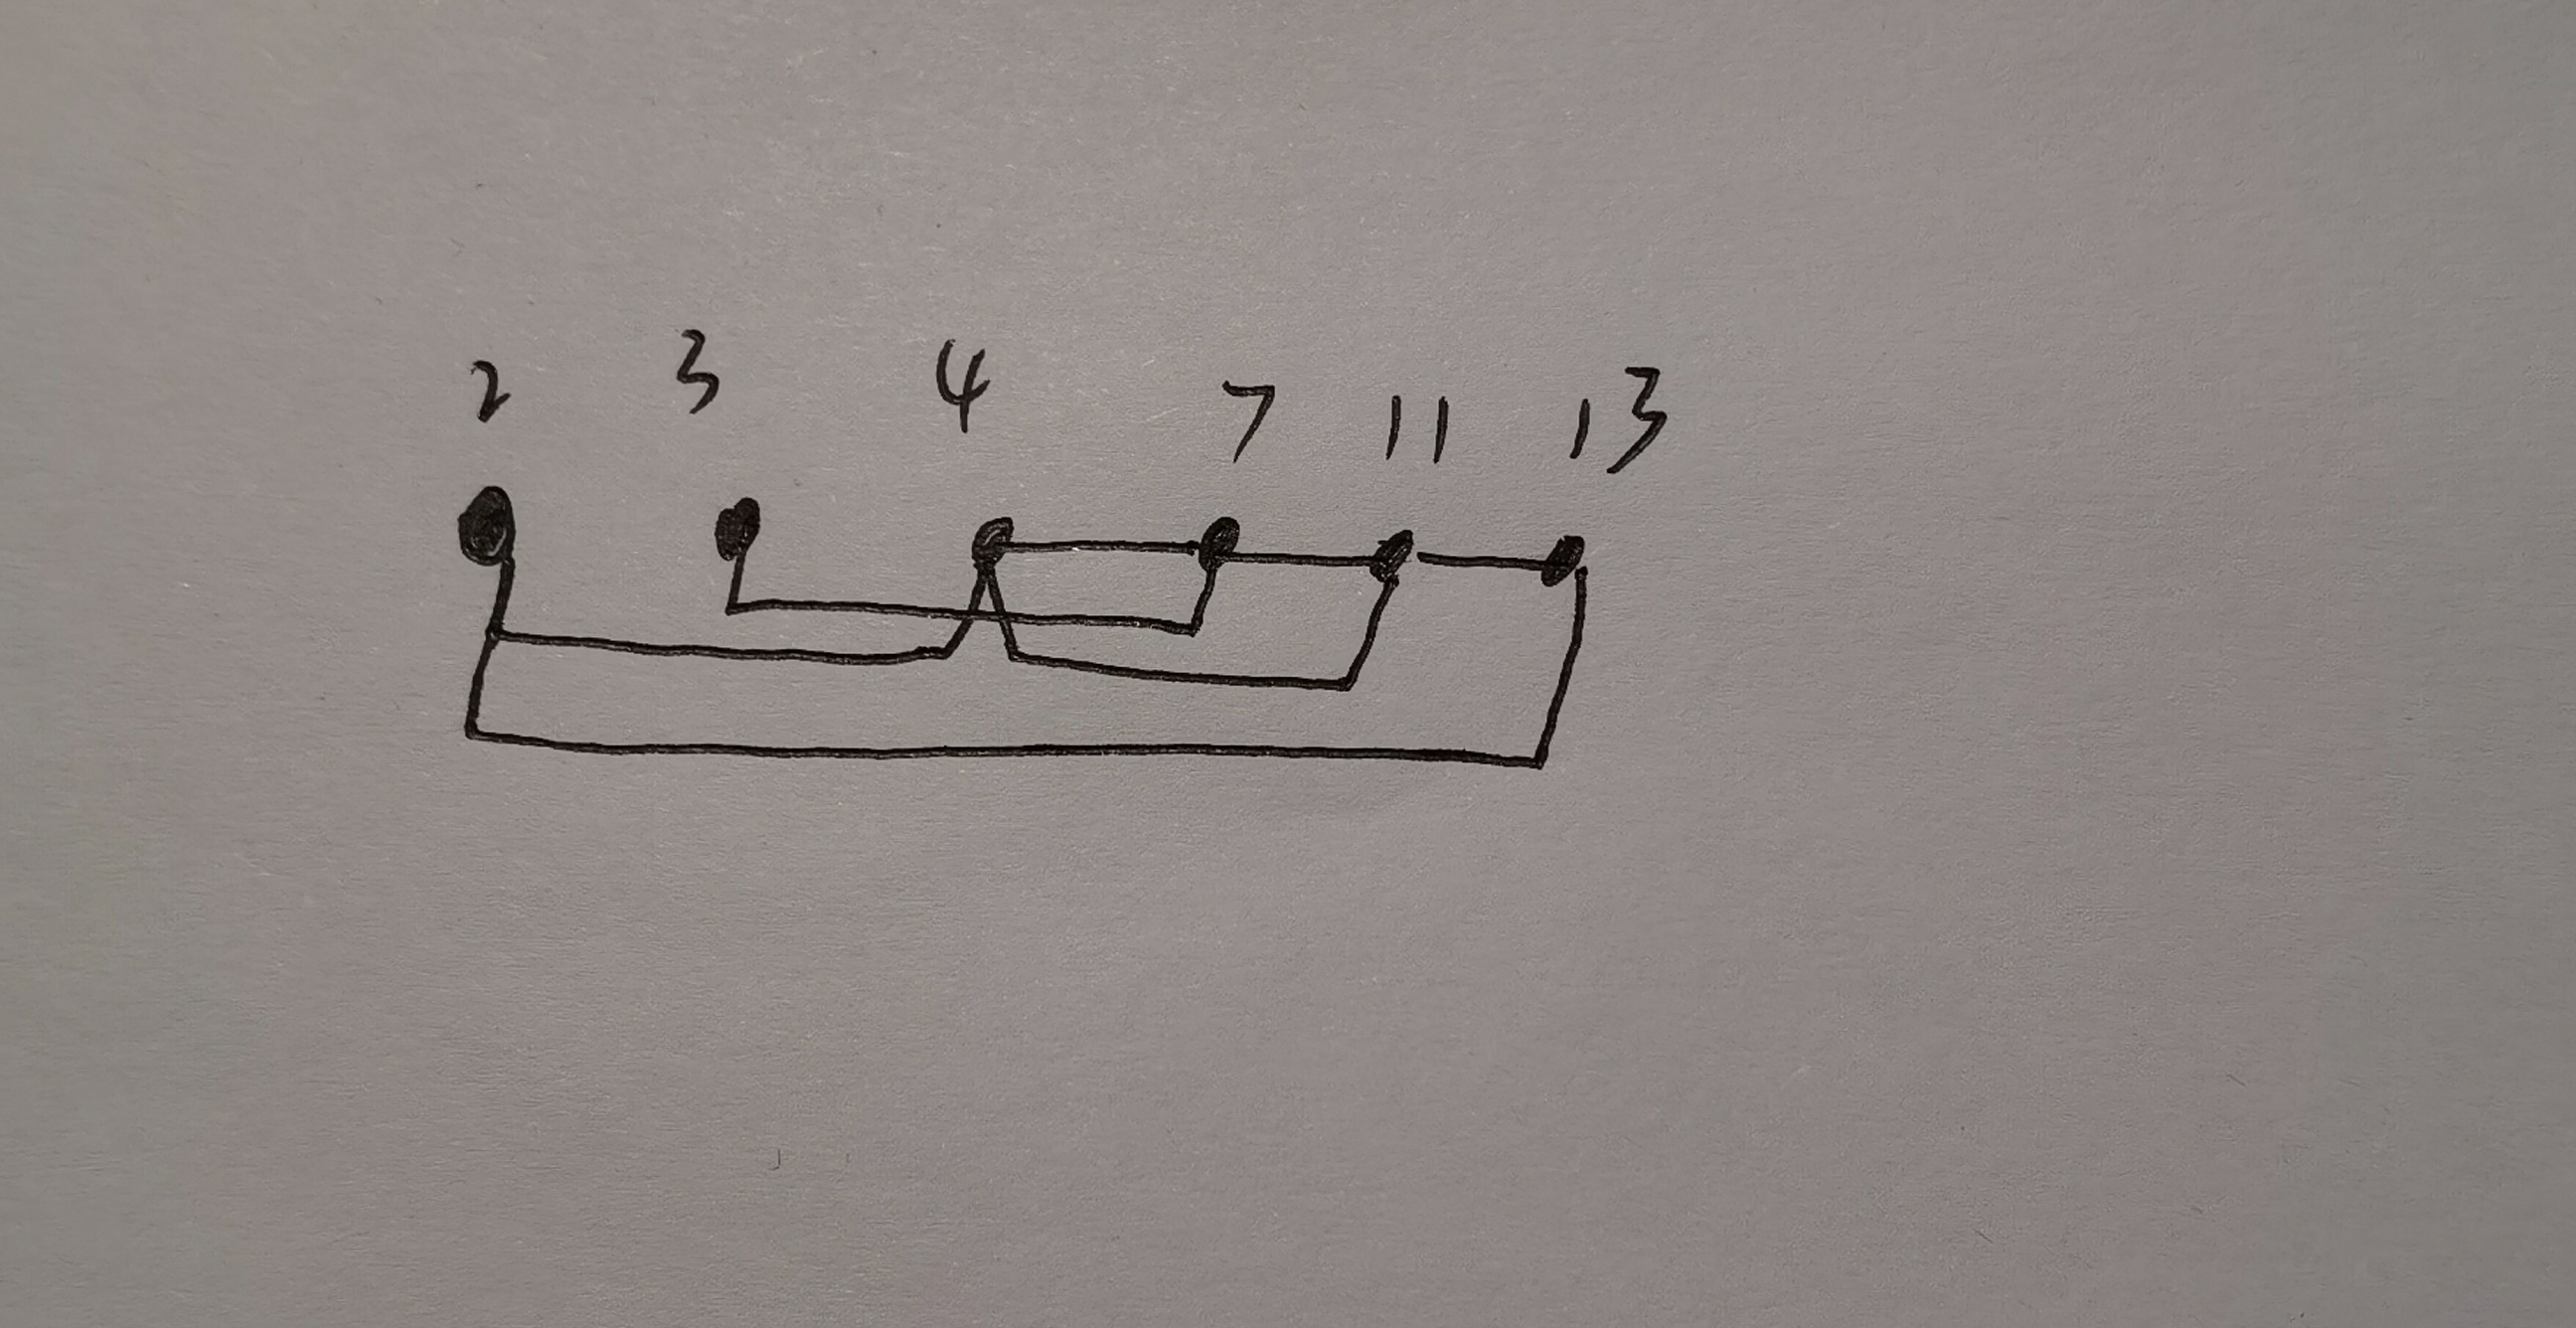
\includegraphics[width = 0.75\linewidth]{fig.jpg}
    \end{figure}

\end{solution}
%%%%%%%%%%%%%%%

%%%%%%%%%%%%%%%
\begin{problem}[3-4.6 CZ 2.1]
Give an example of the following or explain why no such example exists:\\
(a) a graph of order 7 whose vertices have degrees 1, 1, 1, 2, 2, 3, 3. \\
(b) a graph of order 7 whose vertices have degrees 1, 2, 2, 2, 3, 3, 7.\\
(c) a graph of order 4 whose vertices have degrees 1, 3, 3, 3.
\end{problem}

\begin{solution}
    (a) Non-existent. Its sum of degrees is $13$, which is not even and contrary to the first law of graph theory.\\
    (b) Non-existent. For a figure with a point of $7$, the maximum degree is $6$.\\
    (c) Non-existent. A figure with a point of $4$ has a degree of $3$, indicating that if $3$ points are connected to all other points, it is impossible to have a point with a degree of $1$.
\end{solution}

\begin{problem}[3-2.1 TC 16.1-2]
Suppose that instead of always selecting the first activity to finish, we instead select the last activity to start that is compatible with all previously selected activities. De- scribe how this approach is a greedy algorithm, and prove that it yields an optimal solution.
\end{problem}

\begin{solution}
    Assuming that all event intervals are left open and right closed, the algorithm proposed in the textbook is obviously still correct. \\
    Suppose the original $i$ activity starts at $s_i$ and ends at $t_i$
    Let $T=max{t_i}$. \\
    Reset the timeline in reverse order. That is, under the new timeline, the start time of each activity $s^{'}_i=T-t_i$, and the end time $t^{'}_i=T-s_i$\\
    The event time under the original problem is $[s_i,t_i)$, and the event time under the new problem is $(t^{'}_i,s^{'}_i]$\\
    Obviously, for this problem, after conversion, the problem is still the same as the original problem and has the same optimal solution. \\
    After conversion, according to the proven algorithm, the event with the earliest end is prioritized each time. At this point, the event that ended first is the same as the event that first started the original problem. Selecting the event that ends earliest after the transition is equivalent to selecting the event that starts later in the original issue. \\
    Therefore, this approach can still obtain the optimal solution.
\end{solution}
%%%%%%%%%%%%%%%

%%%%%%%%%%%%%%%%%%%%
% 如果没有反馈,可以把这部分删掉
\beginfb

% 你可以写
% ~\footnote{优先推荐 \href{problemoverflow.top}{ProblemOverflow}}:
% \begin{itemize}
%   \item 对课程及教师的建议与意见
%   \item 教材中不理解的内容
%   \item 希望深入了解的内容
%   \item $\cdots$
% \end{itemize}
%%%%%%%%%%%%%%%%%%%%
% \bibliography{2-5-solving-recurrence}
% \bibliographystyle{plainnat}
%%%%%%%%%%%%%%%%%%%%
\end{document}